\documentclass{article}
\usepackage{tikz}
\usetikzlibrary{shapes.geometric,calc,angles,positioning,intersections,quotes,decorations,babel,patterns,fit}
\usepackage{tkz-euclide}
\usetkzobj{all}
\begin{document}
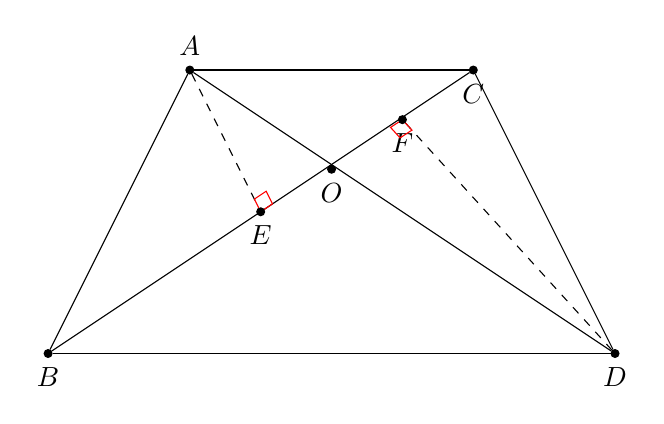
\begin{tikzpicture}
[scale =0.9,>=stealth,point/.style = {draw, circle, fill = black, inner sep = 1pt},]
\node (A) at (2,4)[point,label=above :$A$] {};
\node (B) at (0,0)[point,label=below :$B$] {};
\node (C) at (6,4)[point,label=below :$C$] {};
\node (D) at (8,0)[point,label=below :$D$] {};
\node (E) at (3,2)[point,label=below :$E$] {};
\node (F) at (5,3.3)[point,label=below :$F$] {};
\node (O) at (4,2.6)[point,label=below :$O$] {};
\draw (D)--(A);
\draw (A)--(B);
\draw (B)--(C);
\draw (A)--(C);
\draw (B)--(D);
\draw (C)--(D);
\draw [dashed] (A) -- (E);
\draw [dashed] (D) -- (F);
\tkzMarkRightAngle[draw=red,size=.2](A,E,C)
\tkzMarkRightAngle[draw=red,size=.2](D,F,E)
\end{tikzpicture}
\end{document} 